\documentclass{beamer}

\usepackage[frenchb]{babel}
\usepackage[utf8]{inputenc}

\usetheme{Frankfurt}

\addtobeamertemplate{navigation symbols}{\usebeamerfont{footline}%
	\usebeamercolor[fg]{footline}
	\hspace{1em}
	\insertframenumber/\inserttotalframenumber}

\title[Outil de gestion de parcours-patient]{Outil de gestion de parcours-patient dans un hôpital de jour}
\subtitle{Soutenance de Projet R\&D}
\author{Romain ROUSSEAU}
\date{\today}


\begin{document}
	
\begin{frame}[plain]
	\titlepage
\end{frame}

\AtBeginSection[]
{
\begin{frame}
	
	\tableofcontents[currentsection, hideallsubsections]
	
\end{frame} 
}

\begin{frame}[plain]
\frametitle{Introduction}

Projet Recherche \& Développement sur l'amélioration d'un outil de gestion de parcours-patient pour l'AP-HP (Assistance publique - Hôpitaux de Paris).

\begin{figure}
	
\includegraphics[scale=0.7]{images/LOGO_APHP}
\end{figure}

\end{frame}


\begin{frame}

\frametitle{Sommaire}

\tableofcontents

\end{frame}


\section[Contexte]{Contexte et objectifs}


\begin{frame}
\frametitle{Contexte}

La gestion des patients dans les hôpitaux fait l'objet de nombreux débats dans l'actualité.

\bigbreak

\begin{itemize}
	\item Temps d'attente trop longs pour les patients
	\item Problèmes liés aux ressources disponibles (salles, personnel, ...) 
	\item Problèmes budgétaires
\end{itemize}

Développement des cliniques ambulatoires (aussi appelées Hôpitaux de jour)

\end{frame}

\begin{frame}
\frametitle{Contexte}
	
	L'outil va permettre de gérer un ensemble de patients nécessitant plusieurs activités de soin planifiées sur une journée.
	
	\bigbreak
	
	Un patient suit un "\textbf{parcours de soins}" défini par un ensemble d'activités au sein de l'hôpital.
	
	\bigbreak
	
	Une activité de soin est caractérisée par une durée et un ensemble de ressources. Certaines peuvent avoir des \textbf{contraintes de précédence}. 
	
\end{frame}


\begin{frame}
\frametitle{Contexte du projet}

\begin{block}{Suite de plusieurs projets consécutifs}
	\begin{description}
		\item[Projet SI et R\&D 2015-2016]: par 6 étudiants et Jean Coquelet, modélisation et développement des fonctionnalités de base
		\item[Projet R\&D 2016-2017]: par Guillaume Pochet, planification manuelle des activités
		\item[Projet R\&D 2017-2018]: par Yang Jing, ajout de fonctionnalités de gestion
	\end{description}
\end{block}

\end{frame}

\begin{frame}
\frametitle{Objectifs}

Améliorations générales de la plateforme (corrections de bugs, d'erreurs de conception, de fautes d'orthographe, etc.).

\bigbreak

Implémentation de la planification automatique des activités de soin.

\end{frame}

\section[Description]{Description du projet}

\begin{frame}
\frametitle{Description du projet}

Plateforme web développée en PHP, HTML, Javascript à l'aide du framework CodeIgniter.


\begin{figure}
	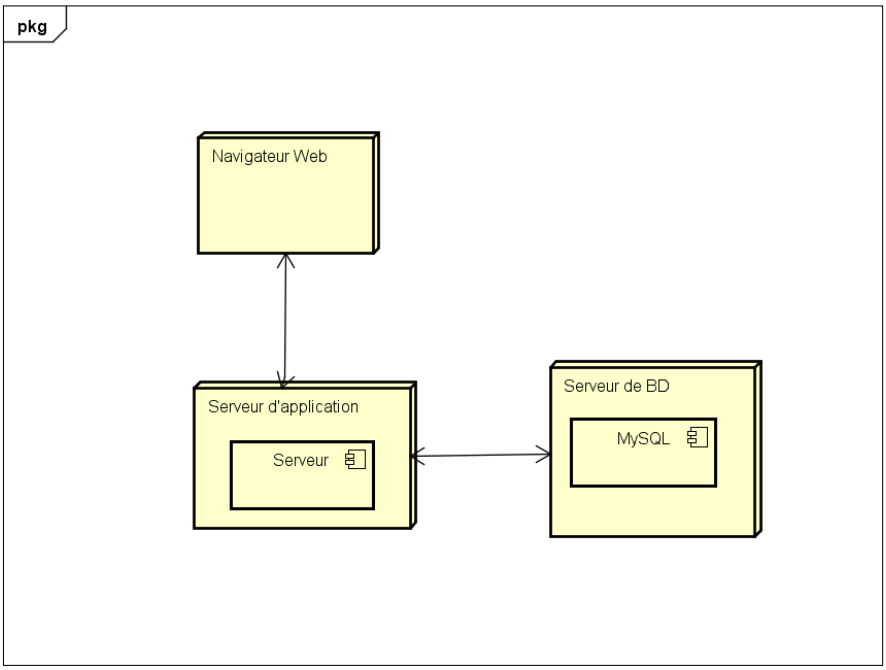
\includegraphics[scale=0.45]{images/deploiement}
\end{figure}

\end{frame}

\begin{frame}
\frametitle{Aperçu de la page d'accueil}

\begin{center}
	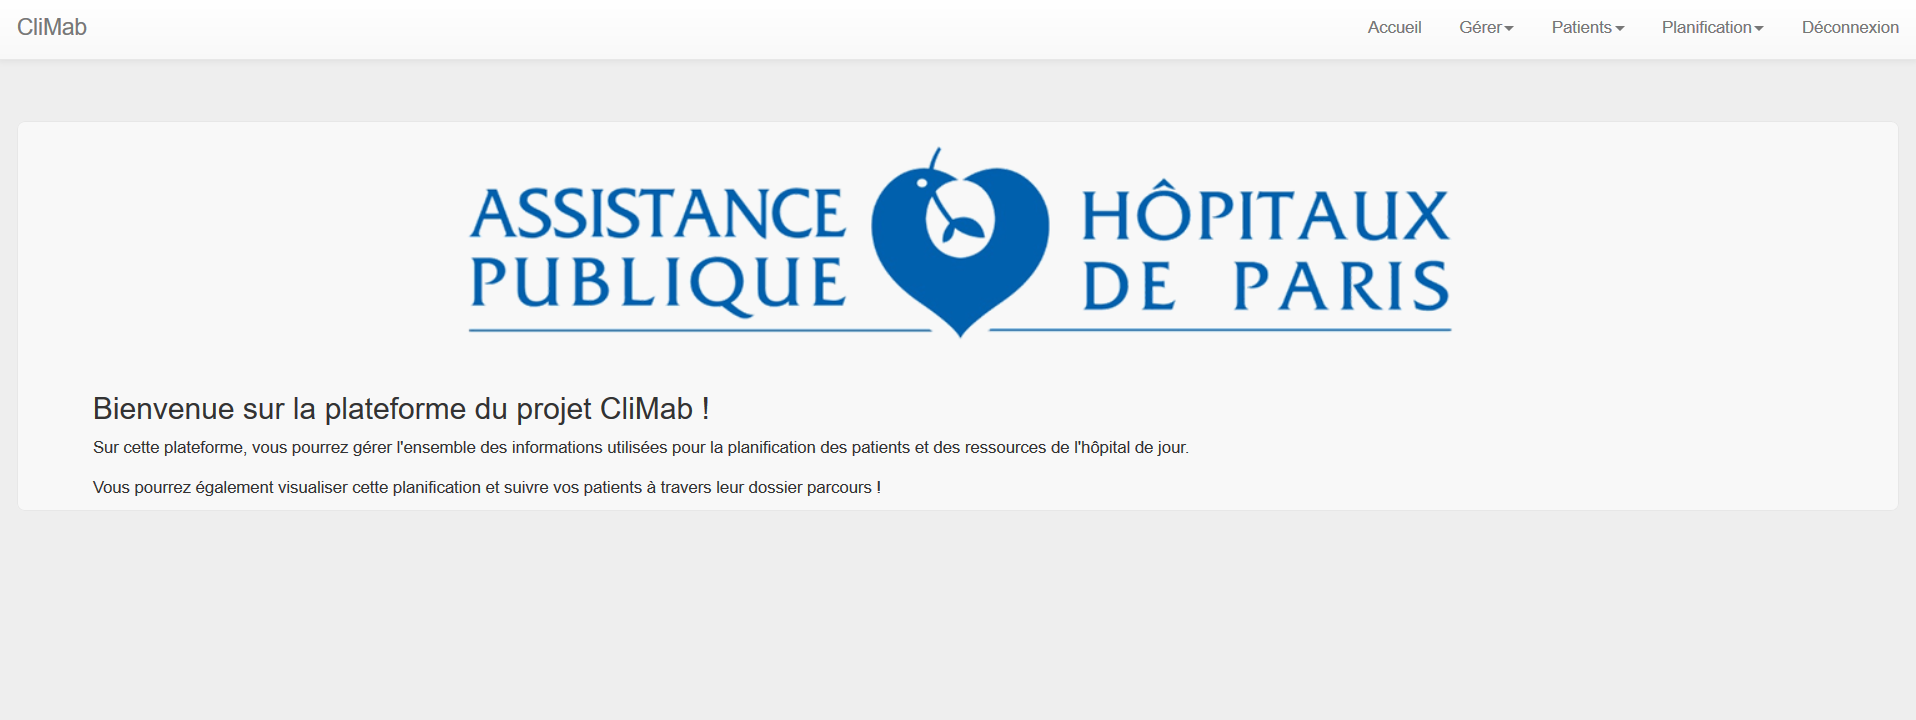
\includegraphics[scale=0.28]{images/accueil}
\end{center}

\end{frame}

\begin{frame}
\frametitle{Onglet de gestion}
	
\begin{center}
	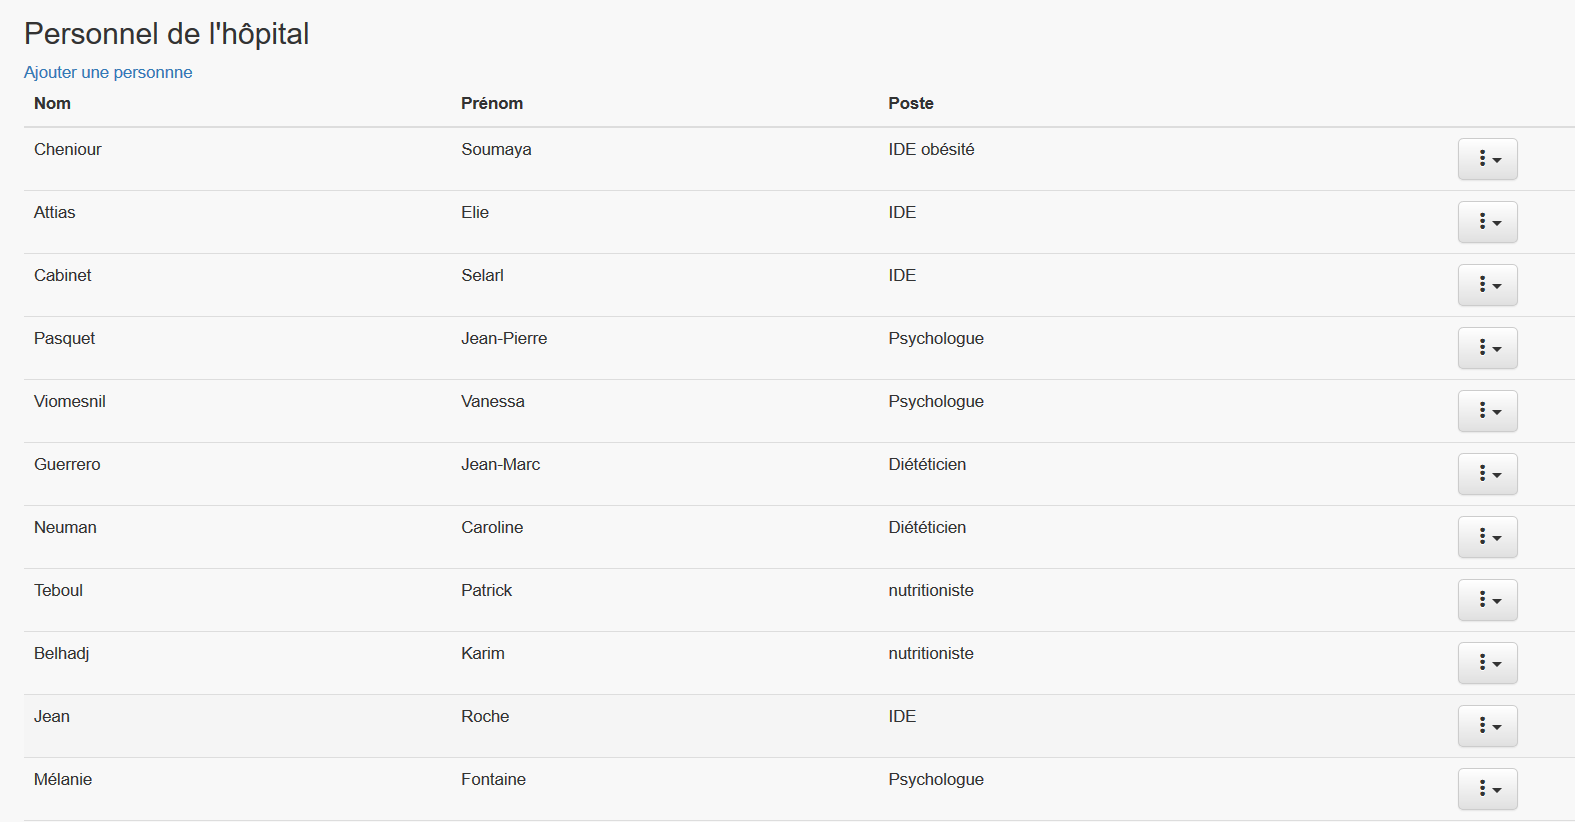
\includegraphics[scale=0.35]{images/affichage_personnel}
\end{center}
	
\end{frame}

\begin{frame}
\frametitle{Onglet "Patient"}

\begin{center}
	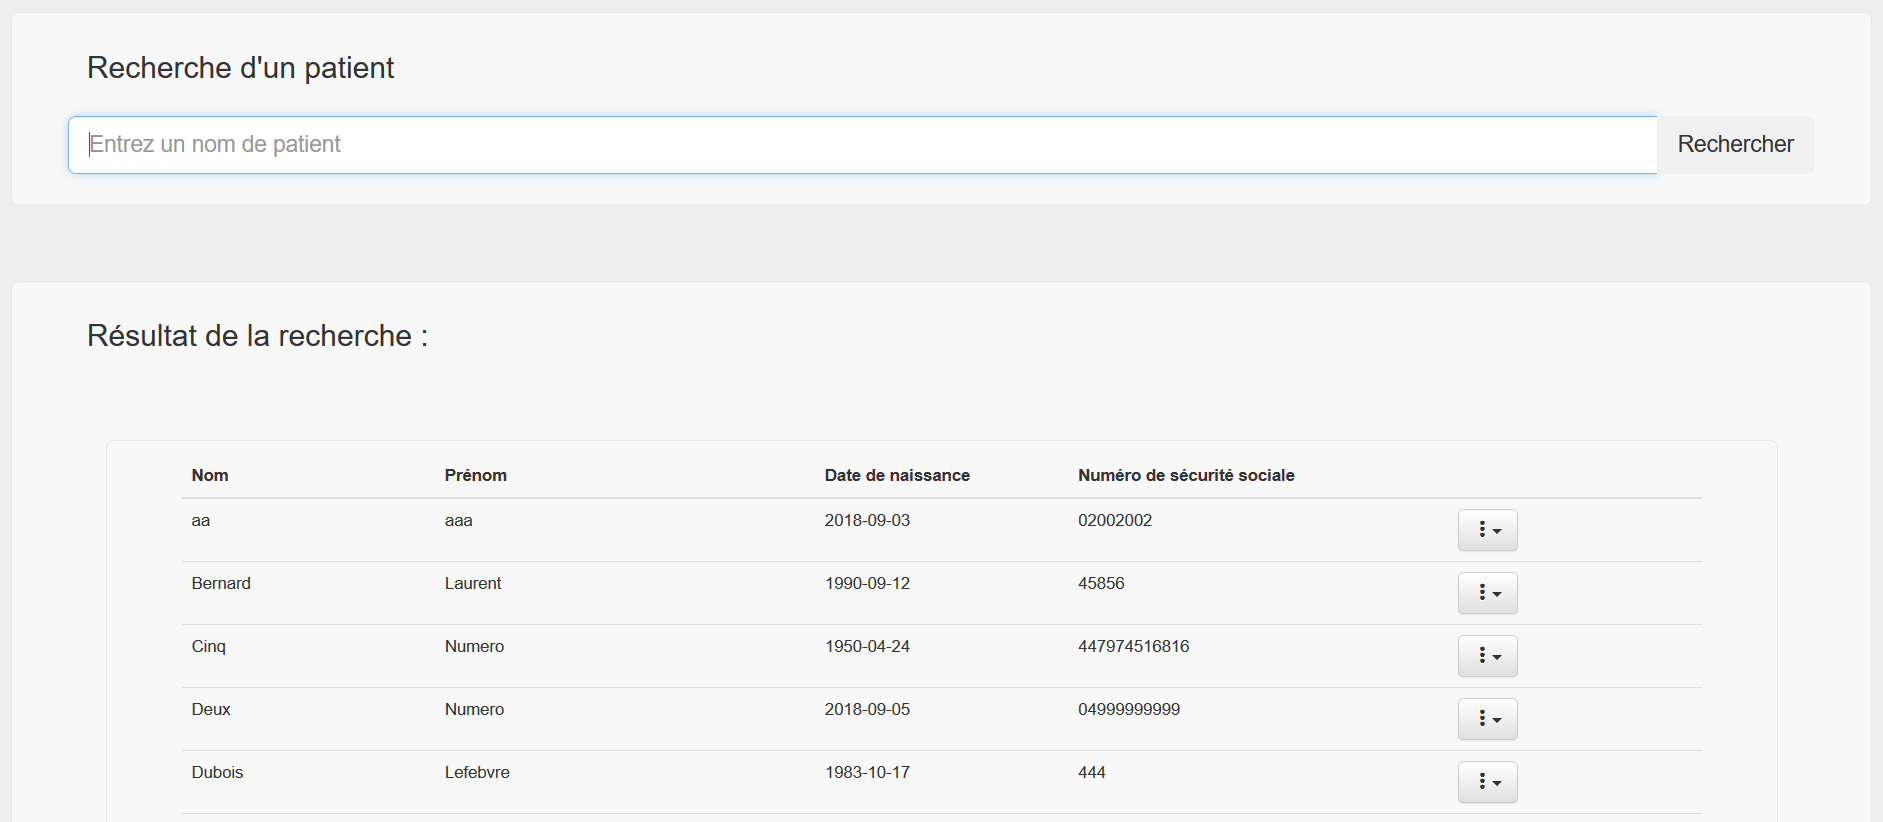
\includegraphics[scale=0.28]{images/recherchePatient}
\end{center}

\end{frame}

\begin{frame}
\frametitle{Onglet de planification}

\begin{center}
	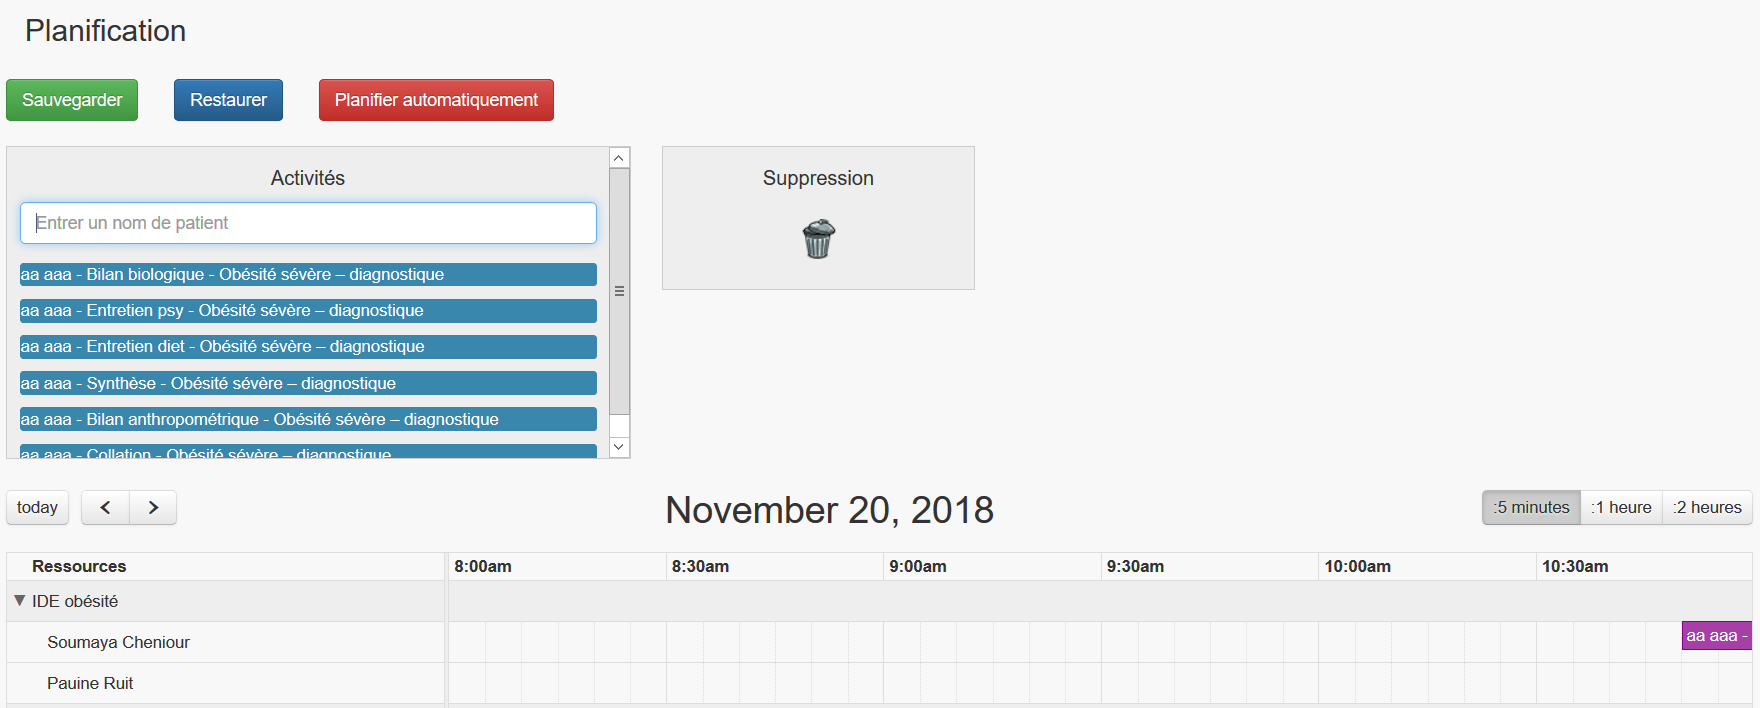
\includegraphics[scale=0.3]{images/bouton_plan_auto}
\end{center}

\end{frame}


\section[Fonctionnalités]{Fonctionnalités à modifier}

\begin{frame}
\frametitle{Fonctionnalités existantes à revoir}

\begin{block}{Revoir la suppression des ressources}
	Aucune sécurité n'était présente sur la suppression des ressources. À minima, un message d'avertissement éviterait les erreurs de manipulation.
\end{block}	

\begin{block}{Revoir le formulaire de création de patient}
	Certains champs ne disposaient d'aucun pré-formattage (exemple: numéro de téléphone sans limite de chiffre)
\end{block}
	
\end{frame}


\begin{frame}
\frametitle{Fonctionnalités existantes à revoir}

\begin{block}{Affichage du planning d'un patient}
	L'affichage du planning pour un patient dans l'onglet "Patient" ne fonctionnait pas.
\end{block}

\begin{block}{Génération de jeux de données pour les tests}
	Un onglet existe mais la fonctionnalité ne fonctionne pas.
\end{block}

\end{frame}


\begin{frame}
\frametitle{Fonctionnalités à ajouter}

\begin{block}{Planification automatique des activités}
	La planification automatique permettrait de générer un planning pour la journée qui, dans l'idéal, réduit le temps d'attente des patients.
\end{block}	

\end{frame}

\section[Gestion de projet]{Gestion de projet}
\begin{frame}
\frametitle{Gestion de projet}

Méthode Agile, un sprint représente chaque fonctionnalité à revoir et/ou à ajouter. 

Chiffrage réalisé au début du projet : $\approx$ 62 jours au total. Fin prévu à la fin du mois de janvier.

\end{frame}

\section*{Conclusion}

\begin{frame}
\frametitle{Conclusion}

La plupart des fonctionnalités à revoir ont été développées (Suppression, les onglets de gestion, etc.). 

\bigbreak

La seconde partie sera consacrée principalement au développement de la planification automatique. 


\end{frame}

\end{document}